\chapter{Temporal Analysis and Ablations}
\label{ch:temporal}

\section{Per-Year Decay}

The temporal protocol trains on 2016--2020 and tests on 2024. Figure~\ref{fig:temporal}
and the full table in Appendix~\ref{app:results} report a per-year view of the
respondent protocol: for each wave from 2016 to 2024, the model is evaluated on
the rows contributed by the 20\% held-out respondents. This holds respondent
identity fixed while letting the year vary.

\begin{figure}[t]
\centering
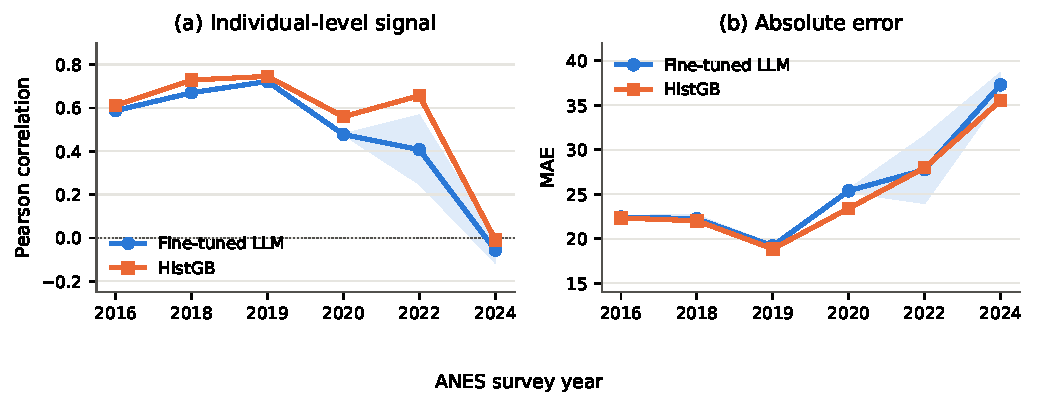
\includegraphics[width=\linewidth]{figures/fig2_temporal_decay.pdf}
\caption{Per-year correlation (a) and MAE (b) for the fine-tuned LLM and HistGB.
Shaded bands are standard deviations over three seeds.}
\label{fig:temporal}
\end{figure}

For the fine-tuned LLM, the correlation is 0.722 in 2019, 0.478 in 2020, 0.408 in
2022, and $-0.056$ in 2024; MAE rises from 19.20 to 25.39, 27.76, and 37.30.
HistGB decays later but collapses in the same way: 0.746, 0.560, 0.657, and
$-0.008$; MAE 18.85, 23.41, 27.98, and 35.52. The decay begins between 2019 and
2020, not at 2024. The LLM decays earlier than the tabular baseline: by 2022 its
correlation is 0.408 while HistGB is still at 0.657.

\section{The 2024 Collapse and a Failed Mitigation}

On the full 2024 test set the fine-tuned LLM reaches an MAE of 36.47 $\pm$ 0.75
but a correlation of $-0.029$ $\pm$ 0.021; HistGB reaches 35.06 and $-0.030$.
The predictions concentrate on the middle of the scale: 3,173 of 3,421 LLM
predictions are exactly 50, and every Biden row is predicted as 50 (standard
deviation 0.0), while Trump rows have a standard deviation of 17.4 and a
correlation of $-0.014$. The anchor readout does not rescue the signal: its
correlation is 0.003 with a prediction standard deviation of 2.1, so its low ECE
is an artefact of near-constant predictions. This is not LLM-specific: HistGB,
which has no language-model component, also loses the individual signal.

A natural mitigation is to add the most recent wave to training. The model is
fine-tuned on the union of the 2016--2020 pool and the 2022 validation rows
(9,017 rows) and evaluated on 2024. The result is unchanged: MAE 36.62,
correlation $-0.030$, choice 0.525. Adding 2022 does not restore the signal,
which points to a genuine distribution shift rather than a lack of recent data.

\section{Ablations}

Three design choices are isolated with matched runs. A1 replaces the nine-strategy
pool with a uniform random sample of the same size. A2 removes the interaction
block from the prompt. A3 additionally removes the candidate's party, position,
and age. All use seed 42 and the same in-distribution rows.

The full model reaches an MAE of 20.84 $\pm$ 0.24, a correlation of 0.679
$\pm$ 0.003, and a choice accuracy of 0.553 $\pm$ 0.011. A1 reaches 21.27, 0.658,
and 0.543; A2 reaches 21.13, 0.670, and 0.567; A3 reaches 21.45, 0.657, and
0.565. The direction is consistent but should be read as a small, descriptive
trend: removing the distribution-aware sampling or the candidate metadata worsens
MAE by roughly half a point and lowers correlation by about 0.02. Because each
ablation uses one seed, the thesis does not claim that each component is
individually necessary; the full table is in Appendix~\ref{app:results}.

The cross-pressure analysis gives a finer-grained view. The fine-tuned LLM is
substantially better than HistGB on CP3, the identity-versus-party conflict (MAE
15.51--17.80 versus 20.31), and comparable on CP1 (18.77--21.55 versus 21.55). It
is slightly worse on CP2 (23.21--24.13 versus 23.18) and on non-conflict rows
(20.45--21.09 versus 20.14). The cells are small, so the result is descriptive.
